\section{zadanie 5}
Zadanie polegało na skorzystaniu z wcześniej zaprogramowanej metody bisekcji w celu znalezienia punktów przecięcia funkcji \[f(x) = 3x\] oraz \[g(x) = e^x\]
Naturalnie, w celu znalezienia punktów przecięcia zajmiemy się szukaniem miejsc zerowych funkcji \[h(x) = f(x) - g(x)\]
Dokładność obliczeń będzie ograniczona przez \(\delta = 10^{-4}\) i \(\epsilon = 10^{-4}\)
\begin{figure}[ht]
  \centering
  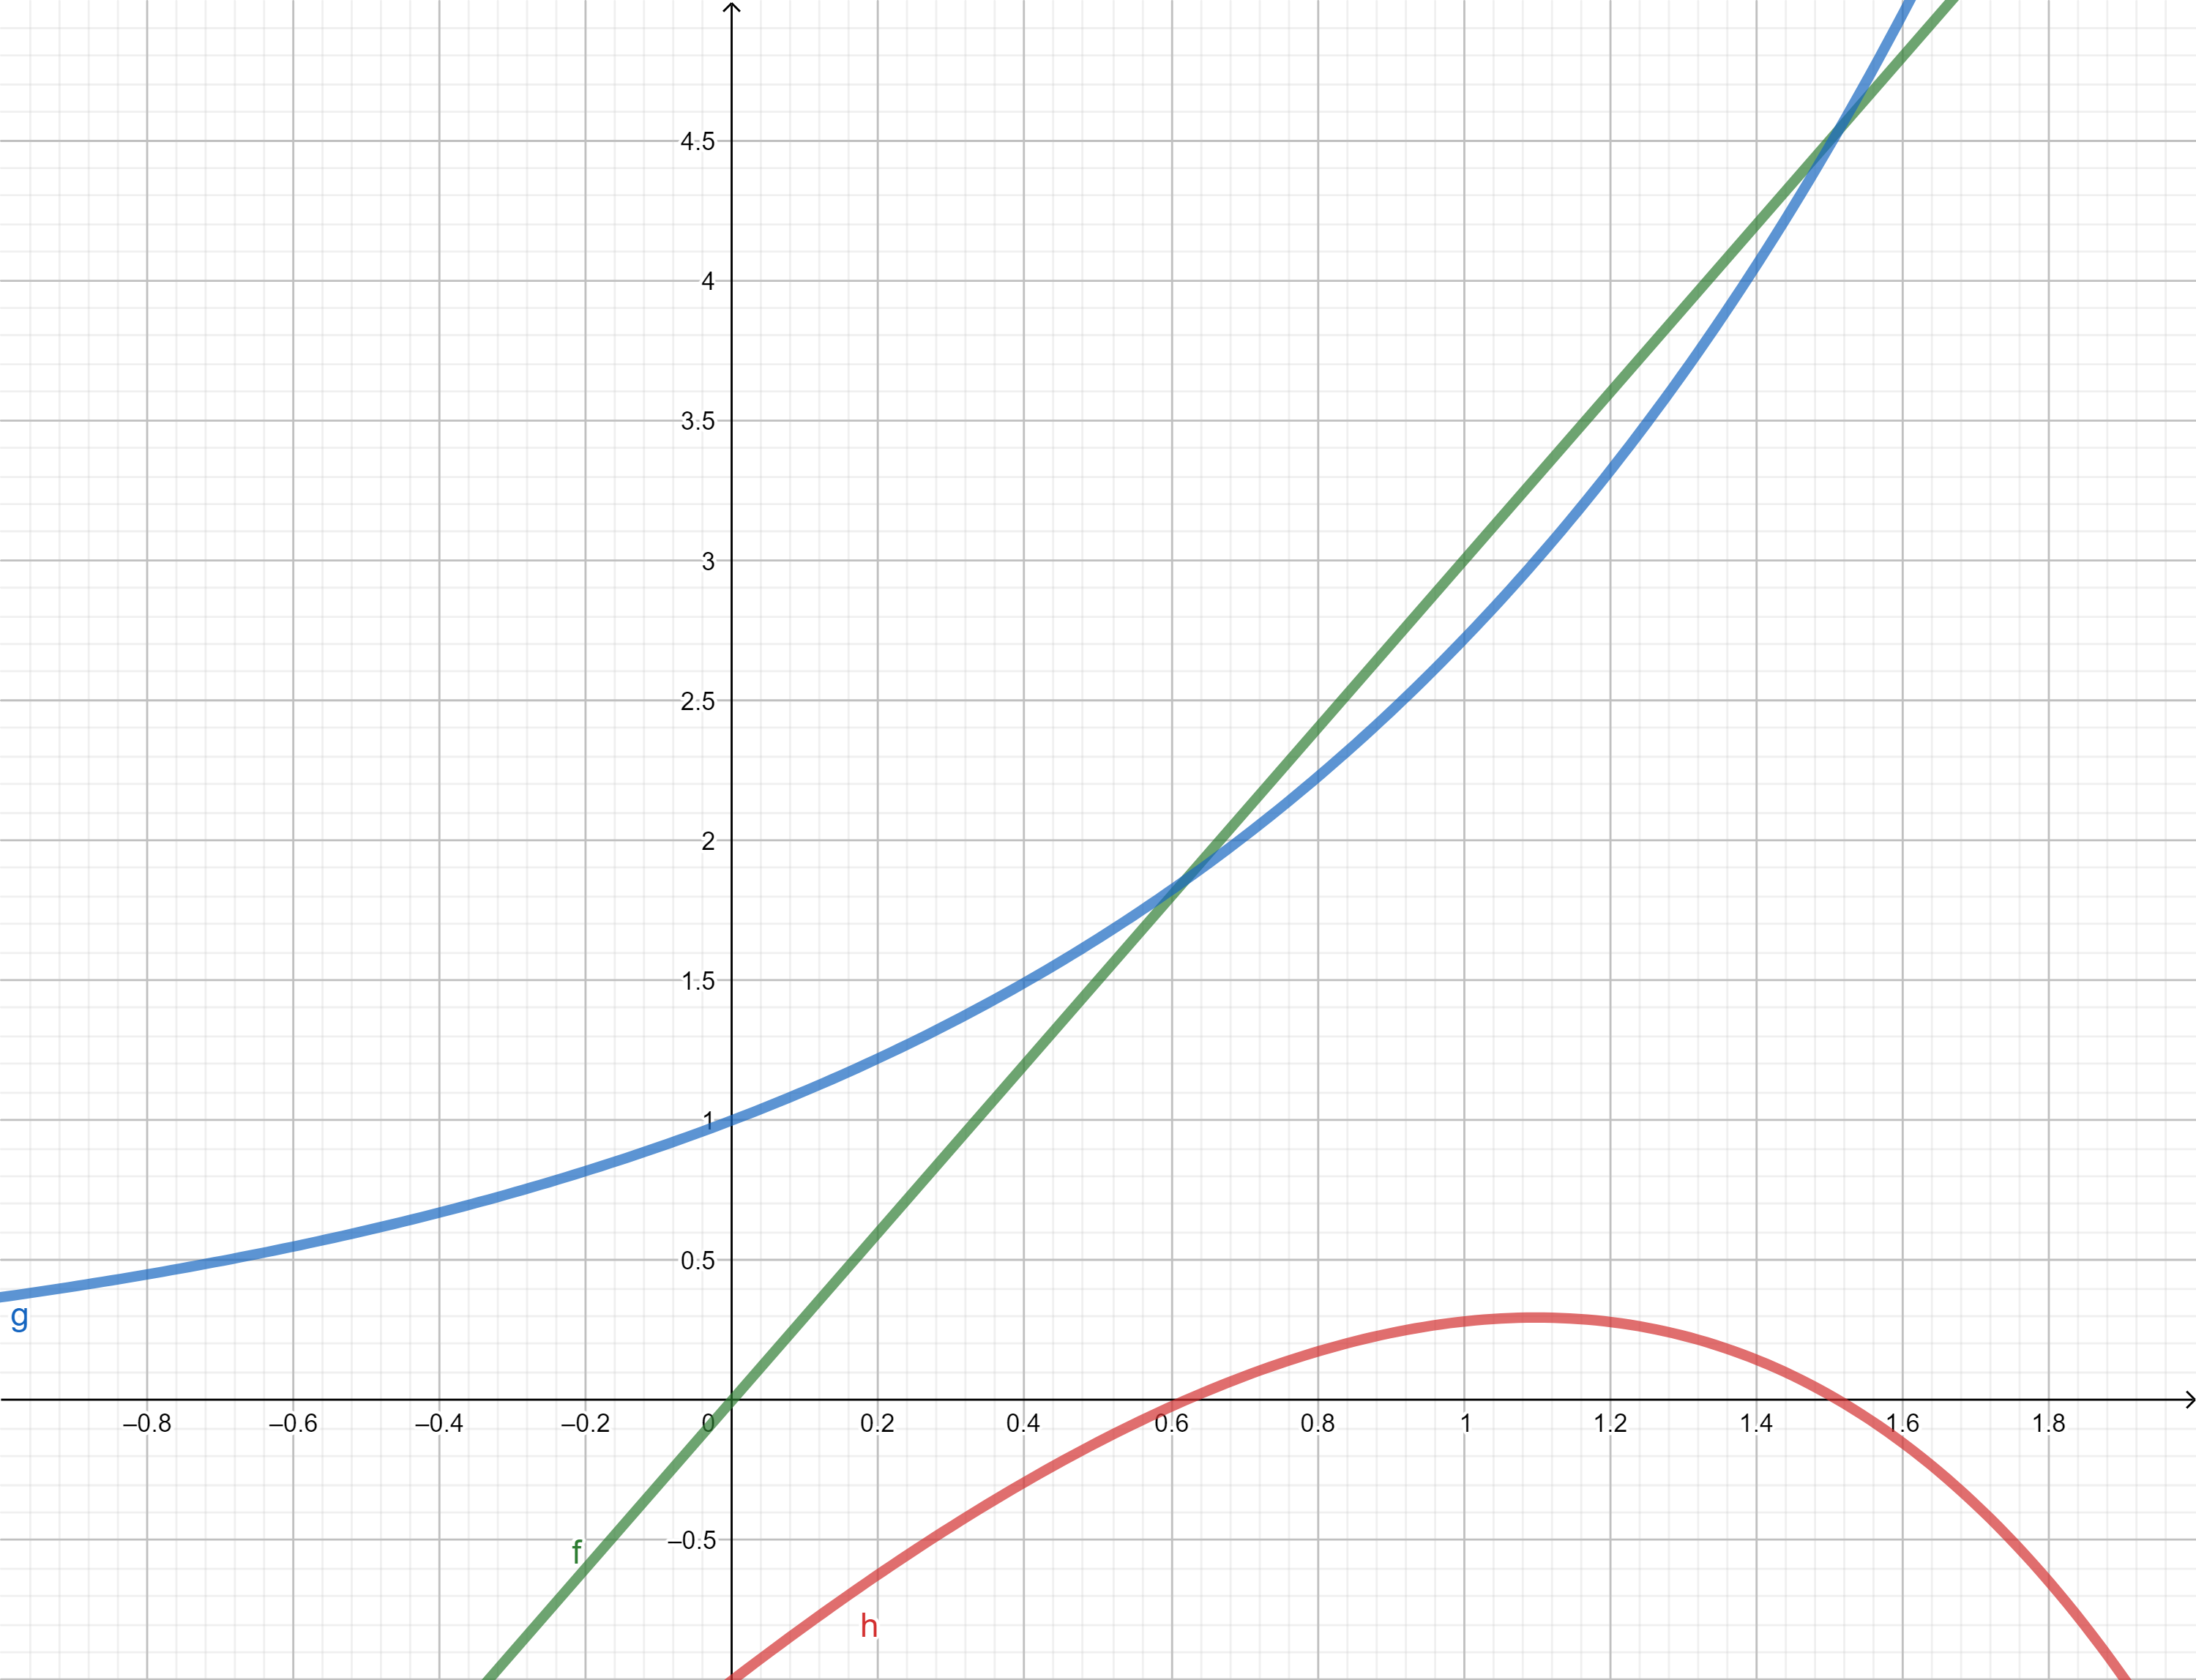
\includegraphics[width=\textwidth]{zadanie5.png}
  \caption{Wykresy funkcji \(f(x)\), \(g(x)\) oraz \(h(x)\)}
\end{figure}


\subsection{Wyniki:}
Wyniki działania programu znajdują się w poniższej tabeli
\begin{table}[ht]
  \makebox[\textwidth]{
    \centering
    \begin{tabular}{|c|c|c|c|c|}
    \hline
    przedział początkowy & \(x\) & \(h(x)\) & iter & error \\
    \hline
    \hline
    \([1.5, 2.0]\) & 1.5120849609375 & 7.618578602741621e-5 & 12 & 0 \\
    \([0.5, 1.0]\) & 0.619140625 & 9.066320343276146e-5 & 8 & 0 \\ 
    \hline
    \end{tabular}
    }
    \caption{wartości z wyjścia programu \textbf{zadanie5.jl}}

\end{table}



\subsection{Wnioski:}
Pomimo że średnice przedziałów były niewielkich rozmiarów metoda bisekcji potrzebowała 8 i 12 iteracji do znalezienia miejsc zerowych z odpowiednią precyzją.